%% =======================================================
%% Actividad 6: Distribuciones empíricas, valores atípicos y datos faltantes
%%
%% Compilar desde actividades/: ./compilar.sh act06
%% Las figuras de img/ se generan con: python act06.py
%% =======================================================

%% ---- CONFIGURACIÓN ------------------------

\documentclass[11pt,letterpaper]{article}

\usepackage[indice]{tecnm}
\usepackage[T1]{fontenc}
\usepackage{amsmath}
\usepackage{xcolor}
\usepackage[most]{tcolorbox} % Carga tcolorbox con soporte para listings y saltos de página
\tcbuselibrary{listings, skins, breakable}
\setlength{\emergencystretch}{3em} % Evita líneas desbordadas por palabras en \texttt

% Paleta de colores (estilo GitHub Light / VS Code)
\definecolor{codebg}{HTML}{F8F9FA}       % Fondo del código
\definecolor{codehead}{HTML}{E9ECEF}     % Fondo de la barra de título
\definecolor{codeborder}{HTML}{CED4DA}   % Borde de la tarjeta
\definecolor{codetitle}{HTML}{212529}    % Texto del título
\definecolor{codekw}{HTML}{0550AE}       % Palabras clave (import, def, for...)
\definecolor{codefunc}{HTML}{8250DF}     % Funciones y métodos (describe, groupby...)
\definecolor{codestr}{HTML}{0A3069}      % Strings
\definecolor{codecomm}{HTML}{6E7781}     % Comentarios
\definecolor{codenum}{HTML}{8C959F}      % Números de línea
\definecolor{codeid}{HTML}{24292F}       % Texto general

% Configuración base de listings
\lstdefinestyle{pythonestilo}{
  language=Python,
  basicstyle=\ttfamily\footnotesize\color{codeid},
  keywordstyle=\color{codekw}\bfseries,
  keywordstyle=[2]\color{codefunc}, % Estilo secundario para métodos de datos
  stringstyle=\color{teal!80!black},
  commentstyle=\color{codecomm}\itshape,
  morekeywords={as, True, False, None, with, yield, lambda},
  morekeywords=[2]{describe, print, len, DataFrame, Series, boxplot, boxplot_stats, hist, plot, axvline, subplots, savefig, tight_layout, concatenate, normal, uniform, choice, seed, mean, median, std, dropna, replace, fillna, isna, sum, round, probplot, pdf, cdf, skew, kurtosis, trim_mean},
  numbers=left,
  numberstyle=\tiny\ttfamily\color{codenum},
  stepnumber=1,
  numbersep=10pt,
  showstringspaces=false,
  morestring=[b]{"""},
  tabsize=4,
  breaklines=true,
  breakatwhitespace=true,
  columns=flexible,
  keepspaces=true,
  literate=
    {á}{{\'a}}1 {é}{{\'e}}1 {í}{{\'i}}1 {ó}{{\'o}}1 {ú}{{\'u}}1
    {Á}{{\'A}}1 {É}{{\'E}}1 {Í}{{\'I}}1 {Ó}{{\'O}}1 {Ú}{{\'U}}1
    {ñ}{{\~n}}1 {Ñ}{{\~N}}1 {¿}{{?`}}1 {¡}{{!`}}1 {±}{{$\pm$}}1
}

% Definición del entorno personalizado \begin{codigo}{Título}{etiqueta}
% \newtcblisting[auto counter, number within=section]{codigo}[2][]{
\newtcblisting[auto counter]{codigo}[2][]{
  listing only,
  breakable,                    % Permite que el bloque se divida si pasa de página
  enhanced,
  colback=codebg,
  colframe=codeborder,
  colbacktitle=codehead,
  coltitle=codetitle,
  fonttitle=\bfseries\small\sffamily,
  boxrule=0.6pt,
  arc=4pt,                      % Bordes redondeados
  left=20pt,                    % Espacio izquierdo para los números de línea
  right=8pt,
  top=6pt,
  bottom=6pt,
  toptitle=4pt,
  bottomtitle=4pt,
  before skip=12pt,
  after skip=12pt,
  listing options={style=pythonestilo},
  title={Código \thetcbcounter: #2},
  #1
}

% Paleta para salida de consola (estilo terminal limpia)
\definecolor{termbg}{HTML}{212529}      % Fondo oscuro tipo terminal
\definecolor{termhead}{HTML}{343A40}    % Barra superior
\definecolor{termtext}{HTML}{F8F9FA}    % Texto claro de alta legibilidad
\definecolor{termborder}{HTML}{495057}  % Borde

% Entorno \begin{consola}[label=out:iris]{Título}
\newtcblisting[auto counter]{consola}[2][]{
  listing only,
  breakable,
  colback=termbg,
  colframe=termborder,
  colbacktitle=termhead,
  coltitle=termtext,
  colupper=termtext,
  fonttitle=\bfseries\small\sffamily,
  boxrule=0.6pt,
  arc=4pt,
  left=8pt,
  right=8pt,
  top=6pt,
  bottom=6pt,
  toptitle=4pt,
  bottomtitle=4pt,
  before skip=12pt,
  after skip=12pt,
  listing options={
    basicstyle=\ttfamily\scriptsize\color{termtext}, % \scriptsize evita que las tablas de Pandas se partan de línea
    breaklines=true,
    columns=fixed,        % Mantiene alineadas las columnas de Pandas
    keepspaces=true,
    showstringspaces=false,
    literate=
      {á}{{\'a}}1 {é}{{\'e}}1 {í}{{\'i}}1 {ó}{{\'o}}1 {ú}{{\'u}}1
      {Á}{{\'A}}1 {É}{{\'E}}1 {Í}{{\'I}}1 {Ó}{{\'O}}1 {Ú}{{\'U}}1
      {ñ}{{\~n}}1 {Ñ}{{\~N}}1 {±}{{$\pm$}}1
  },
  title={Salida \thetcbcounter: #2},
  #1
}

%% ---- DATOS DE LA MATERIA ------------------------

\materia{Modelos Estadísticos para el Aprendizaje \\ Automático y Ciencia de Datos}
\actividad{Tema 1.5
Identificación de Distribuciones Empíricas, Valores Atípicos y Datos Faltantes \\ Actividad 6 - Ejercicios Prácticos}

\profesor{Dr. José Ismael Ojeda Campaña}
%\fecha{15 de octubre de 2026}    % opcional; por defecto es la fecha de hoy

\begin{document}
\portada
\indicegeneral

%% ---- CONTENIDO ---------------------------------

\section{Introducción}

En el análisis de datos no todo lo que se observa refleja fielmente la realidad. Los conjuntos de datos suelen presentar irregularidades que, si no se identifican y tratan, llevan a interpretaciones erróneas y a modelos sesgados. Por eso, antes de aplicar cualquier modelo estadístico o de aprendizaje automático, es necesario estudiar la distribución empírica de los datos, detectar los valores atípicos y tratar correctamente los datos faltantes \parencite{tecnm2026_documento_fuente}.

En este documento se resuelven los tres ejercicios prácticos del tema 1.5, uno por cada uno de esos aspectos. En el primero se compara la distribución empírica de la altura de 200 estudiantes con una distribución normal teórica. En el segundo se analiza cómo dos sueldos de directivos muy altos afectan la media y la mediana de los sueldos de una empresa. En el tercero se estudia el efecto de registrar como cero las respuestas faltantes de una encuesta de ingresos, y se compara con dos tratamientos correctos: excluir los datos faltantes e imputarlos. Como el cuaderno de trabajo no proporciona los datos, en los tres ejercicios se simularon en Python de acuerdo con las condiciones de cada enunciado.

\section{Marco conceptual}

\subsection{Distribuciones empíricas}

Una distribución empírica se obtiene a partir de los valores medidos de una variable aleatoria en un experimento. Al agruparse en un histograma, esos valores forman la distribución de la muestra, que refleja la frecuencia con que ocurre cada valor observado \parencite{tecnm2026_documento_fuente,bonamente2017}. A medida que aumenta el número de mediciones, se espera que la distribución empírica se aproxime a la distribución teórica o \textit{parent distribution}, como la normal o la de Poisson, que representa el modelo ideal de la variable aleatoria \parencite{bonamente2017}. Analizar la distribución empírica es fundamental para entender la naturaleza de las variables y para seleccionar los métodos estadísticos apropiados \parencite{tecnm2026_documento_fuente}.

La distribución normal con media $\mu$ y desviación estándar $\sigma$ tiene la función de densidad
\begin{equation}
    f(x) = \frac{1}{\sigma\sqrt{2\pi}} \exp\!\left(-\frac{(x - \mu)^2}{2\sigma^2}\right),
\end{equation}
que es simétrica respecto a $\mu$ y concentra cerca del 68\,\%, 95\,\% y 99.7\,\% de los valores a una, dos y tres desviaciones estándar de la media, respectivamente \parencite{bonamente2017}. Para comparar una muestra con esta distribución, además del histograma puede usarse un gráfico Q-Q (cuantil-cuantil), que enfrenta los cuantiles de la muestra con los de la distribución teórica: si la muestra es normal, los puntos quedan sobre una línea recta \parencite{bruce2020}.

\subsection{Valores atípicos}

Los valores atípicos (\textit{outliers}) son valores alejados de la media o del centro de la distribución. Pueden deberse a errores de medición, datos faltantes, corrupción de los datos o eventos raros, y pueden distorsionar la distribución y afectar la estimación de sus parámetros \parencite{tecnm2026_documento_fuente,brownlee2019}. Cuando se detectan es importante revisarlos con cuidado, porque pueden indicar problemas experimentales o la necesidad de considerar modelos alternativos \parencite{tecnm2026_documento_fuente}.

Las medidas de tendencia central reaccionan de forma distinta ante los valores atípicos. La media usa el valor de todas las observaciones, por lo que un solo valor extremo puede desplazarla mucho. La mediana solo depende del valor central de los datos ordenados, por lo que es una medida \textbf{robusta}: casi no cambia ante valores extremos \parencite{bruce2020}. Una alternativa intermedia es la media recortada, que descarta un porcentaje fijo de los valores más bajos y más altos antes de promediar \parencite{bruce2020}.

Un criterio común para detectar valores atípicos es el del diagrama de caja, que considera atípico todo valor menor que $Q_1 - 1.5\,\text{RIC}$ o mayor que $Q_3 + 1.5\,\text{RIC}$, donde $\text{RIC} = Q_3 - Q_1$ es el rango intercuartílico \parencite{bruce2020}.

\subsection{Datos faltantes}

Los datos faltantes son una causa común de distorsión en la distribución, especialmente cuando se codifican como ceros u otros valores arbitrarios. Esto puede introducir artificialmente valores extremos o modificar la forma de la distribución \parencite{tecnm2026_documento_fuente,brownlee2019}. La limpieza de datos (\textit{data cleaning}) incluye la detección de valores atípicos y la imputación, que consiste en reparar o rellenar los valores faltantes con métodos estadísticos, por ejemplo con la media o la mediana de los valores observados \parencite{tecnm2026_documento_fuente,brownlee2019}. En \texttt{pandas}, los datos faltantes se representan con \texttt{NaN}, se cuentan con \texttt{isna()}, se eliminan con \texttt{dropna()} y se imputan con \texttt{fillna()} \parencite{tecnm2026_documento_fuente}.

\section{Descripción de la actividad}

\textbf{Objetivo:} Analizar distribuciones empíricas, valores atípicos y datos faltantes, y cuantificar su efecto sobre la forma de la distribución y las medidas de tendencia central.

Los ejercicios del cuaderno de trabajo son los siguientes \parencite{tecnm2026_documento_fuente}:

\begin{description}
    \item[Ejercicio 1.] Medir la altura (en cm) de 200 estudiantes, construir un histograma y comparar visualmente la distribución empírica con una distribución normal teórica.
    \item[Ejercicio 2.] Registrar los sueldos mensuales de 100 empleados, donde la mayoría gana entre \$15,000 y \$30,000 pero 2 directivos ganan más de \$150,000. Calcular la media y la mediana de los sueldos y analizar cómo estos valores atípicos afectan las medidas de tendencia central.
    \item[Ejercicio 3.] En una encuesta sobre ingresos mensuales, el 15\,\% de los participantes no respondió y sus valores aparecen como 0. Calcular la media de los ingresos con y sin esos ceros y analizar cómo afecta la distribución empírica.
\end{description}

\section{Desarrollo}

Los tres ejercicios se resolvieron en el script \texttt{act06.py}, que usa \texttt{numpy}, \texttt{pandas}, \texttt{matplotlib} y \texttt{scipy.stats}. Los datos se simularon con semillas aleatorias fijas para que los resultados sean reproducibles. Cada figura se guarda como imagen PNG en la carpeta \texttt{img/}. El Código~\ref{cod:comun} contiene las importaciones y dos funciones auxiliares: \texttt{guardar()}, que guarda la figura actual y la muestra en pantalla cuando el código se ejecuta en un cuaderno, y \texttt{resumen()}, que calcula las medidas de tendencia central y dispersión de una muestra ignorando los valores \texttt{NaN}. El cuaderno interactivo puede consultarse en Google Colab:

\begin{center}
    \url{https://colab.research.google.com/drive/13yDJkPHB9cuHjkGte3rXYNKvSCK_xXdk?usp=sharing}
\end{center}

\begin{codigo}[label=cod:comun]{Importaciones y funciones auxiliares}
import os

import matplotlib

# En Colab o Jupyter no existe __file__; ahí las figuras también se muestran en pantalla
EN_NOTEBOOK = '__file__' not in globals()
if not EN_NOTEBOOK:
    matplotlib.use('Agg')  # Como script, genera las figuras como archivos PNG sin abrir ventanas

import matplotlib.pyplot as plt
import numpy as np
import pandas as pd
from matplotlib.cbook import boxplot_stats
from scipy import stats

# Carpeta donde se guardan las figuras que se incluyen en el reporte
BASE = os.getcwd() if EN_NOTEBOOK else os.path.dirname(os.path.abspath(__file__))
CARPETA_IMG = os.path.join(BASE, 'img')
os.makedirs(CARPETA_IMG, exist_ok=True)


def guardar(nombre):
    """Guarda la figura actual en la carpeta img/ y la muestra si se ejecuta en un notebook."""
    plt.tight_layout()
    plt.savefig(os.path.join(CARPETA_IMG, nombre), dpi=150)
    if EN_NOTEBOOK:
        plt.show()
    plt.close()


def resumen(datos):
    """Medidas de tendencia central y dispersión de una muestra."""
    datos = pd.Series(datos).dropna()
    return {'n': len(datos), 'Media': datos.mean(), 'Mediana': datos.median(),
            'Desv. est.': datos.std(), 'Mínimo': datos.min(), 'Máximo': datos.max()}
\end{codigo}

\subsection{Ejercicio 1: Distribución empírica de la altura}

Las alturas de los 200 estudiantes se simularon con una distribución normal de media 165\,cm y desviación estándar 8\,cm, redondeadas a 0.1\,cm como si se hubieran medido con cinta. La distribución normal teórica se construyó con la media y la desviación estándar estimadas a partir de la propia muestra.

El histograma se dibujó con \texttt{density=True}, de modo que el área total de las barras es 1 y puede compararse directamente con la curva de densidad normal. Como extensiones, se agregaron un gráfico Q-Q con \texttt{stats.probplot()}, el cálculo de la asimetría y la curtosis de la muestra, y una comparación entre el porcentaje de datos a una, dos y tres desviaciones estándar de la media y el que predice la distribución normal.

\begin{codigo}[label=cod:ej1]{Ejercicio 1: altura de 200 estudiantes}
# Las alturas se simulan con una distribución normal de media 165 cm y
# desviación estándar 8 cm, redondeadas a 0.1 cm como si se midieran con cinta
np.random.seed(15)
alturas = np.round(np.random.normal(165, 8, 200), 1)

# Parámetros de la normal teórica estimados a partir de la muestra
mu, sigma = alturas.mean(), alturas.std(ddof=1)

fig, (ax1, ax2) = plt.subplots(1, 2, figsize=(11, 4.5))

# Histograma de densidad (área total = 1) con la curva normal teórica encima
ax1.hist(alturas, bins=15, density=True, color='skyblue', edgecolor='black',
         label='Distribución empírica')
x = np.linspace(alturas.min() - 5, alturas.max() + 5, 200)
ax1.plot(x, stats.norm.pdf(x, mu, sigma), color='red', linewidth=2,
         label=f'Normal teórica\n($\\mu$ = {mu:.1f}, $\\sigma$ = {sigma:.1f})')
ax1.set_title('Altura de 200 estudiantes')
ax1.set_xlabel('Altura (cm)')
ax1.set_ylabel('Densidad')
ax1.legend(fontsize=8)
ax1.grid(axis='y', linestyle='--', alpha=0.6)

# Gráfico Q-Q: si los puntos siguen la recta, la muestra se parece a la normal
stats.probplot(alturas, dist='norm', plot=ax2)
ax2.get_lines()[0].set(markerfacecolor='skyblue', markeredgecolor='navy', markersize=4)
ax2.get_lines()[1].set(color='red', linewidth=2)
ax2.set_title('Gráfico Q-Q contra la distribución normal')
ax2.set_xlabel('Cuantiles teóricos')
ax2.set_ylabel('Cuantiles de la muestra (cm)')
ax2.grid(linestyle='--', alpha=0.6)
guardar('ej1_altura.png')

# Proporción de datos a 1, 2 y 3 desviaciones estándar de la media
regla = pd.DataFrame({
    'Muestra (%)': [np.mean(np.abs(alturas - mu) <= k * sigma) * 100 for k in (1, 2, 3)],
    'Normal (%)': [(stats.norm.cdf(k) - stats.norm.cdf(-k)) * 100 for k in (1, 2, 3)],
}, index=['± 1 sigma', '± 2 sigma', '± 3 sigma']).round(1)

print("=== Ejercicio 1: altura de 200 estudiantes ===")
print(pd.Series(resumen(alturas)).round(2).to_string())
print(f"Asimetría: {stats.skew(alturas):.3f}")
print(f"Curtosis (exceso): {stats.kurtosis(alturas):.3f}")
print("\nDatos dentro de k desviaciones estándar de la media:")
print(regla)
\end{codigo}

\subsection{Ejercicio 2: Valores atípicos en los sueldos}

Se simularon 98 sueldos con una distribución uniforme entre \$15,000 y \$30,000, redondeados a decenas, y se agregaron dos sueldos de directivos de \$158,000 y \$175,000. La media, la mediana y la media recortada al 5\,\% se calcularon con y sin los directivos para medir el efecto de los valores atípicos. Como extensión, los directivos no se marcaron a mano como atípicos: se detectaron con la regla de $1.5\,\text{RIC}$ mediante \texttt{boxplot\_stats()}, y se calculó cuántos empleados ganan menos que la media.

\begin{codigo}[label=cod:ej2]{Ejercicio 2: sueldos de 100 empleados}
# 98 empleados ganan entre $15,000 y $30,000; 2 directivos ganan más de $150,000
np.random.seed(25)
sueldos_empleados = np.round(np.random.uniform(15_000, 30_000, 98), -1)
sueldos_directivos = np.array([158_000, 175_000])
sueldos = np.concatenate([sueldos_empleados, sueldos_directivos])

# Detección de valores atípicos con la regla de 1.5 veces el rango intercuartílico
caja = boxplot_stats(sueldos)[0]
atipicos = caja['fliers']

comparacion = pd.DataFrame({
    'Con directivos': resumen(sueldos),
    'Sin directivos': resumen(sueldos_empleados),
}).T
comparacion['Media recortada 5%'] = [stats.trim_mean(sueldos, 0.05),
                                     stats.trim_mean(sueldos_empleados, 0.05)]

fig, (ax1, ax2) = plt.subplots(1, 2, figsize=(11, 4.5),
                               gridspec_kw={'width_ratios': [2, 1]})

ax1.hist(sueldos, bins=30, color='lightgreen', edgecolor='black')
ax1.axvline(sueldos.mean(), color='red', linestyle='--', linewidth=2,
            label=f'Media: ${sueldos.mean():,.0f}')
ax1.axvline(np.median(sueldos), color='blue', linewidth=2,
            label=f'Mediana: ${np.median(sueldos):,.0f}')
ax1.set_title('Sueldos mensuales de 100 empleados')
ax1.set_xlabel('Sueldo mensual (pesos)')
ax1.set_ylabel('Número de empleados')
ax1.xaxis.set_major_formatter(matplotlib.ticker.StrMethodFormatter('${x:,.0f}'))
ax1.tick_params(axis='x', labelrotation=20)
ax1.legend()
ax1.grid(axis='y', linestyle='--', alpha=0.6)

ax2.boxplot(sueldos, tick_labels=['Todos'], patch_artist=True, showmeans=True,
            boxprops=dict(facecolor='lightgreen'),
            meanprops=dict(marker='D', markerfacecolor='red', markeredgecolor='red'))
ax2.set_title('Diagrama de caja')
ax2.yaxis.set_major_formatter(matplotlib.ticker.StrMethodFormatter('${x:,.0f}'))
ax2.grid(axis='y', linestyle='--', alpha=0.6)
guardar('ej2_sueldos.png')

print("\n=== Ejercicio 2: sueldos de 100 empleados ===")
print(comparacion.round(0).astype(int).T)
print(f"\nLímite superior para atípicos (Q3 + 1.5 RIC): "
      f"${caja['q3'] + 1.5 * caja['iqr']:,.0f}")
print(f"Valores atípicos detectados: {[f'${v:,.0f}' for v in atipicos]}")
cambio_media = sueldos.mean() - sueldos_empleados.mean()
cambio_mediana = np.median(sueldos) - np.median(sueldos_empleados)
print(f"Efecto de los directivos sobre la media: +${cambio_media:,.0f} "
      f"({cambio_media / sueldos_empleados.mean():.1%})")
print(f"Efecto de los directivos sobre la mediana: +${cambio_mediana:,.0f} "
      f"({cambio_mediana / np.median(sueldos_empleados):.1%})")
print(f"Empleados que ganan menos que la media: {(sueldos < sueldos.mean()).sum()} de 100")
\end{codigo}

\subsection{Ejercicio 3: Datos faltantes codificados como cero}

Se simularon los ingresos mensuales reales de 200 participantes con una distribución normal de media \$18,000 y desviación estándar \$4,000. Después se eligieron al azar 30 participantes (el 15\,\%) y su ingreso se reemplazó por 0, para reproducir la base de datos descrita en el enunciado. Al haber simulado los datos, se conocen los ingresos reales de todos los participantes, lo que permite evaluar qué tan cerca queda cada tratamiento del valor verdadero.

Se compararon cuatro versiones de la variable:

\begin{enumerate}
    \item \textbf{Con ceros:} la base de datos tal como está, tratando los ceros como ingresos reales.
    \item \textbf{Sin ceros:} los ceros se convierten en \texttt{NaN} con \texttt{replace(0, np.nan)} y se excluyen de los cálculos.
    \item \textbf{Imputado:} como extensión, los \texttt{NaN} se rellenan con la mediana de los ingresos observados mediante \texttt{fillna()}.
    \item \textbf{Valores reales:} los ingresos simulados antes de introducir los faltantes, que sirven como referencia.
\end{enumerate}

\begin{codigo}[label=cod:ej3]{Ejercicio 3: ingresos con respuestas faltantes}
# Ingresos reales de 200 participantes (en pesos)
np.random.seed(35)
ingresos_reales = np.round(np.random.normal(18_000, 4_000, 200), -1)

# El 15% no respondió y en la base de datos aparece como 0
encuesta = pd.DataFrame({'ingreso': ingresos_reales})
no_respondieron = np.random.choice(encuesta.index, size=int(0.15 * len(encuesta)), replace=False)
encuesta.loc[no_respondieron, 'ingreso'] = 0

# Tratamiento correcto: los ceros son datos faltantes, no ingresos de $0
encuesta['ingreso_na'] = encuesta['ingreso'].replace(0, np.nan)
print("\n=== Ejercicio 3: ingresos con respuestas faltantes ===")
print(f"Participantes: {len(encuesta)}")
print(f"Respuestas registradas como 0: {(encuesta['ingreso'] == 0).sum()}")
print(f"Datos faltantes tras convertir 0 a NaN: {encuesta['ingreso_na'].isna().sum()}")

# Imputación por la mediana de los ingresos observados
mediana_obs = encuesta['ingreso_na'].median()
encuesta['ingreso_imputado'] = encuesta['ingreso_na'].fillna(mediana_obs)

comparacion = pd.DataFrame({
    'Con ceros': resumen(encuesta['ingreso']),
    'Sin ceros (NaN)': resumen(encuesta['ingreso_na']),
    'Imputado (mediana)': resumen(encuesta['ingreso_imputado']),
    'Valores reales': resumen(ingresos_reales),
})
print()
print(comparacion.round(0).astype(int))
error = encuesta['ingreso'].mean() - ingresos_reales.mean()
print(f"\nError de la media con ceros respecto a la real: ${error:,.0f} "
      f"({error / ingresos_reales.mean():.1%})")

fig, axes = plt.subplots(1, 3, figsize=(13, 4.2), sharey=True)
bins = np.arange(0, 32_001, 2_000)
paneles = [
    (encuesta['ingreso'], 'Con ceros', 'salmon'),
    (encuesta['ingreso_na'].dropna(), 'Sin ceros (faltantes excluidos)', 'skyblue'),
    (encuesta['ingreso_imputado'], 'Imputado con la mediana', 'plum'),
]
for ax, (datos, titulo, color) in zip(axes, paneles):
    ax.hist(datos, bins=bins, color=color, edgecolor='black')
    ax.axvline(datos.mean(), color='red', linestyle='--', linewidth=2,
               label=f'Media: ${datos.mean():,.0f}')
    ax.axvline(datos.median(), color='blue', linewidth=1.5,
               label=f'Mediana: ${datos.median():,.0f}')
    ax.set_title(titulo)
    ax.set_xlabel('Ingreso mensual (pesos)')
    ax.xaxis.set_major_formatter(matplotlib.ticker.StrMethodFormatter('${x:,.0f}'))
    ax.tick_params(axis='x', labelrotation=30)
    ax.legend(fontsize=8)
    ax.grid(axis='y', linestyle='--', alpha=0.6)
axes[0].set_ylabel('Número de participantes')
guardar('ej3_ingresos.png')

print(f"\nFiguras guardadas en {os.path.basename(CARPETA_IMG)}/")
\end{codigo}

\section{Resultados}

\subsection{Ejercicio 1: Distribución empírica de la altura}

\begin{figure}[htbp]
\centering
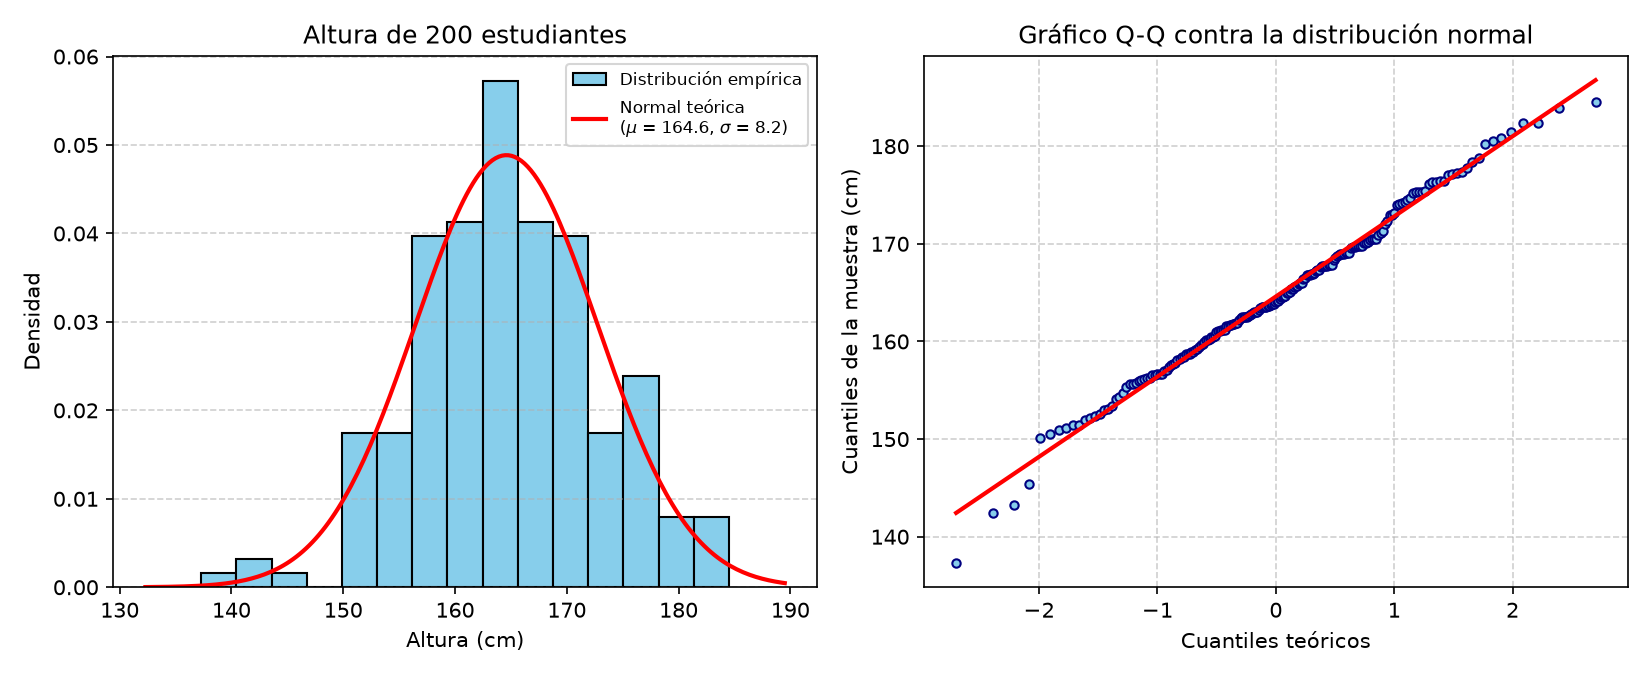
\includegraphics[width=\textwidth]{img/ej1_altura.png}
\caption{Izquierda: histograma de densidad de la altura de 200 estudiantes con la distribución normal teórica. Derecha: gráfico Q-Q de la muestra contra la distribución normal.}
\label{fig:altura}
\end{figure}

\begin{consola}[label=out:ej1]{Ejecución de \texttt{act06.py}: Ejercicio 1}
=== Ejercicio 1: altura de 200 estudiantes ===
n             200.00
Media         164.60
Mediana       164.05
Desv. est.      8.17
Mínimo        137.30
Máximo        184.50
Asimetría: -0.071
Curtosis (exceso): 0.259

Datos dentro de k desviaciones estándar de la media:
           Muestra (%)  Normal (%)
± 1 sigma         68.5        68.3
± 2 sigma         95.5        95.4
± 3 sigma         99.5        99.7
\end{consola}

\begin{itemize}
    \item \textbf{Forma general.} La Figura~\ref{fig:altura} muestra que la distribución empírica tiene la forma de campana de la normal teórica ($\mu = 164.6$\,cm, $\sigma = 8.2$\,cm): es unimodal, con el pico alrededor de 165\,cm, y las frecuencias disminuyen de forma gradual hacia ambos lados.
    \item \textbf{Simetría.} La media (164.60\,cm) y la mediana (164.05\,cm) difieren en apenas medio centímetro, y la asimetría es prácticamente nula ($-0.071$). La curtosis en exceso de 0.259 también es cercana a 0, el valor de la distribución normal.
    \item \textbf{Proporciones.} Los porcentajes de datos a una, dos y tres desviaciones estándar de la media (68.5\,\%, 95.5\,\% y 99.5\,\%) coinciden casi exactamente con los de la normal (68.3\,\%, 95.4\,\% y 99.7\,\%).
    \item \textbf{Diferencias.} La distribución empírica no es idéntica a la teórica: algunas barras del histograma quedan por encima o por debajo de la curva, por ejemplo en el pico central. Estas diferencias son la variación aleatoria natural de una muestra finita. En el gráfico Q-Q los puntos siguen la recta casi en todo el rango y solo se separan en la cola inferior, donde los estudiantes más bajos (el mínimo es de 137.3\,cm) están un poco más lejos de la media de lo que predice la normal.
\end{itemize}

En conjunto, los datos son consistentes con una distribución normal. Esto coincide con lo que plantea la teoría: con un número suficiente de mediciones, la distribución empírica se aproxima a la distribución teórica de la variable \parencite{bonamente2017}.

\subsection{Ejercicio 2: Valores atípicos en los sueldos}

\begin{figure}[htbp]
\centering
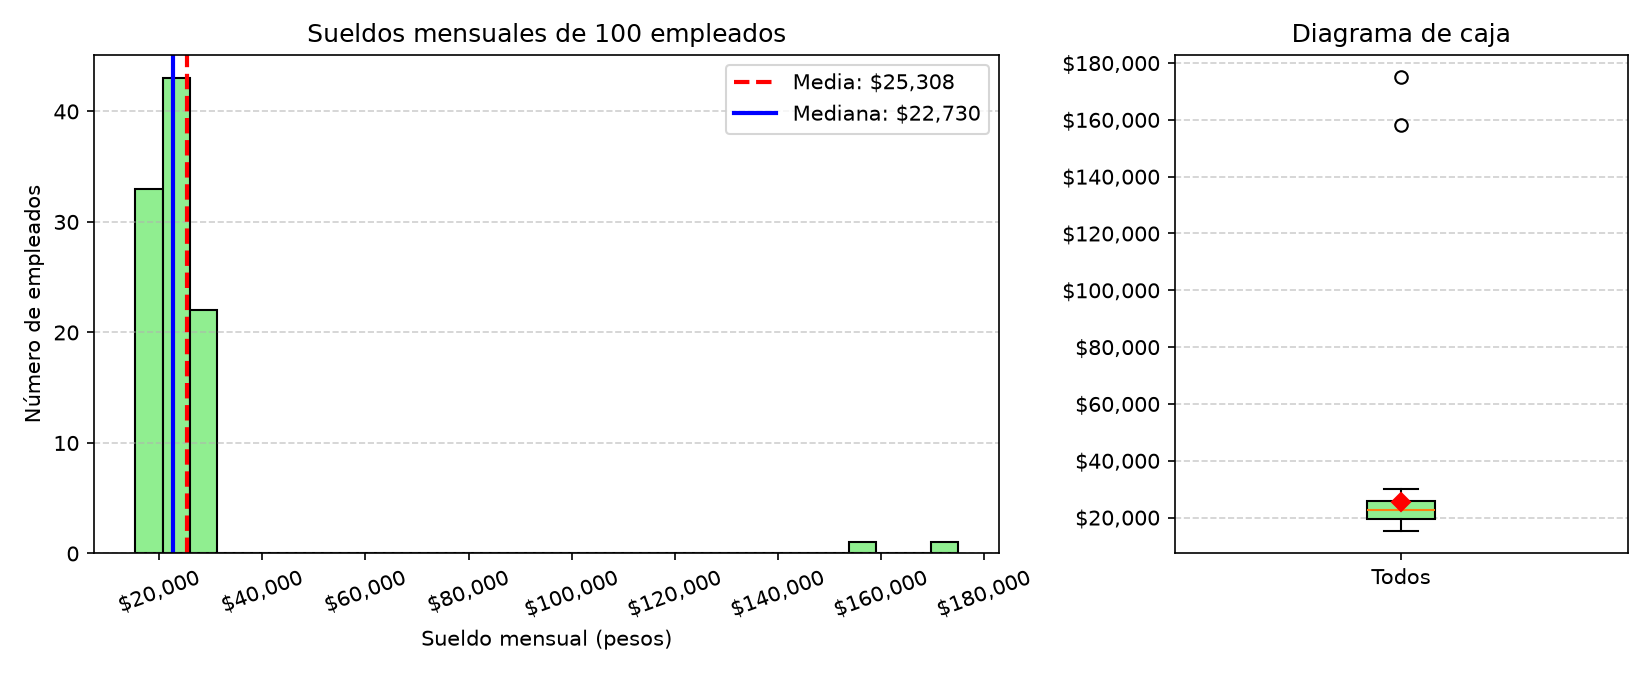
\includegraphics[width=\textwidth]{img/ej2_sueldos.png}
\caption{Histograma y diagrama de caja de los sueldos mensuales de 100 empleados. Los dos sueldos de los directivos aparecen como valores atípicos.}
\label{fig:sueldos}
\end{figure}

\begin{consola}[label=out:ej2]{Ejecución de \texttt{act06.py}: Ejercicio 2}
=== Ejercicio 2: sueldos de 100 empleados ===
                    Con directivos  Sin directivos
n                              100              98
Media                        25308           22427
Mediana                      22730           22700
Desv. est.                   20690            3999
Mínimo                       15320           15320
Máximo                      175000           29960
Media recortada 5%           22572           22433

Límite superior para atípicos (Q3 + 1.5 RIC): $35,366
Valores atípicos detectados: ['$158,000', '$175,000']
Efecto de los directivos sobre la media: +$2,881 (12.8%)
Efecto de los directivos sobre la mediana: +$30 (0.1%)
Empleados que ganan menos que la media: 71 de 100
\end{consola}

La Tabla~\ref{tab:sueldos} resume el efecto de los directivos sobre cada medida.

\begin{table}[htbp]
\centering
\caption{Efecto de los sueldos de los directivos sobre las medidas de tendencia central.}
\label{tab:sueldos}
\begin{tabular}{lrrr}
\hline
\textbf{Medida} & \textbf{Con directivos} & \textbf{Sin directivos} & \textbf{Cambio} \\
\hline
Media              & \$25,308 & \$22,427 & +12.8\,\% \\
Mediana            & \$22,730 & \$22,700 & +0.1\,\% \\
Media recortada 5\,\% & \$22,572 & \$22,433 & +0.6\,\% \\
Desviación estándar & \$20,690 & \$3,999 & +417\,\% \\
\hline
\end{tabular}
\end{table}

\begin{itemize}
    \item \textbf{Detección.} La regla de $1.5\,\text{RIC}$ fija el límite superior en \$35,366 e identifica como atípicos exactamente los dos sueldos de los directivos. En el diagrama de caja de la Figura~\ref{fig:sueldos} aparecen muy por encima del resto, que queda comprimido en una caja pequeña.
    \item \textbf{Efecto sobre la media.} Solo 2 de 100 sueldos bastan para subir la media en \$2,881, un 12.8\,\%. Con los directivos, la media (\$25,308) deja de representar un sueldo típico: 71 de los 100 empleados ganan menos que ella.
    \item \textbf{Efecto sobre la mediana.} La mediana apenas cambia, solo \$30 (0.1\,\%), porque depende de los valores centrales y no del tamaño de los extremos. Lo mismo ocurre con la media recortada al 5\,\%, que al descartar los valores más altos y más bajos cambia solo un 0.6\,\%.
    \item \textbf{Efecto sobre la dispersión.} La desviación estándar es la medida más afectada: pasa de \$3,999 a \$20,690, más de cinco veces mayor, porque eleva al cuadrado las distancias a la media.
\end{itemize}

Para describir el sueldo típico de esta empresa, la mediana es la medida adecuada. Los sueldos de los directivos no son errores, sino valores reales que pertenecen a un grupo distinto, por lo que no deben eliminarse sin más. Lo recomendable es reportarlos por separado o usar medidas robustas, como la mediana, para describir al conjunto \parencite{tecnm2026_documento_fuente,bruce2020}.

\subsection{Ejercicio 3: Datos faltantes codificados como cero}

\begin{figure}[htbp]
\centering
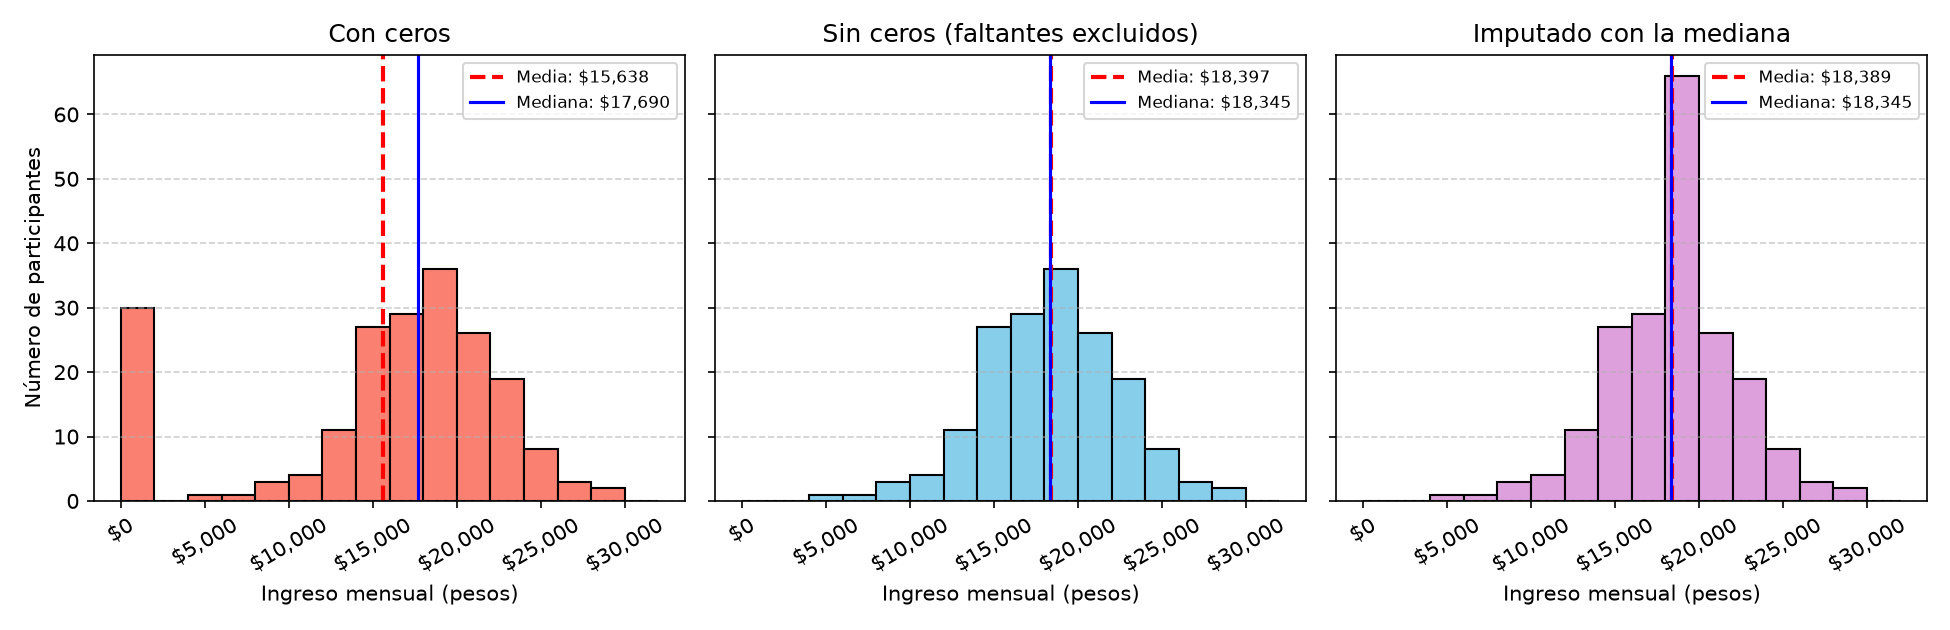
\includegraphics[width=\textwidth]{img/ej3_ingresos.png}
\caption{Histogramas de los ingresos mensuales con los faltantes registrados como 0 (izquierda), excluidos (centro) e imputados con la mediana (derecha).}
\label{fig:ingresos}
\end{figure}

\begin{consola}[label=out:ej3]{Ejecución de \texttt{act06.py}: Ejercicio 3}
=== Ejercicio 3: ingresos con respuestas faltantes ===
Participantes: 200
Respuestas registradas como 0: 30
Datos faltantes tras convertir 0 a NaN: 30

            Con ceros  Sin ceros (NaN)  Imputado (mediana)  Valores reales
n                 200              170                 200             200
Media           15638            18397               18389           18222
Mediana         17690            18345               18345           18215
Desv. est.       7622             4164                3837            4293
Mínimo              0             5930                5930            5930
Máximo          29370            29370               29370           29370

Error de la media con ceros respecto a la real: $-2,584 (-14.2%)

Figuras guardadas en img/
\end{consola}

\begin{itemize}
    \item \textbf{Media con y sin ceros.} Con los ceros, la media de los ingresos es de \$15,638; al excluirlos, sube a \$18,397. Tratar los ceros como ingresos reales subestima la media en \$2,584, un 14.2\,\% por debajo de la media real (\$18,222). El error es casi del mismo tamaño que el porcentaje de faltantes, porque cada cero arrastra el promedio hacia abajo.
    \item \textbf{Efecto en la distribución empírica.} El histograma con ceros (Figura~\ref{fig:ingresos}, izquierda) muestra una barra artificial de 30 participantes en \$0, separada del resto de los datos, cuyo ingreso más bajo es de \$5,930. La distribución pasa de ser aproximadamente simétrica a tener una cola izquierda: la media (\$15,638) queda claramente por debajo de la mediana (\$17,690), y la desviación estándar casi se duplica, de \$4,293 a \$7,622. Los ceros introducen valores extremos que en realidad no existen.
    \item \textbf{Exclusión de faltantes.} Al convertir los ceros en \texttt{NaN} y excluirlos, la distribución recupera su forma simétrica y la media (\$18,397) y la mediana (\$18,345) quedan a menos de \$200 de los valores reales. El costo es trabajar con 170 respuestas en lugar de 200.
    \item \textbf{Imputación con la mediana.} Imputar conserva las 200 observaciones y deja la media (\$18,389) muy cerca de la real. Sin embargo, coloca los 30 valores imputados exactamente en \$18,345, lo que crea un pico artificial en el histograma (Figura~\ref{fig:ingresos}, derecha) y reduce la desviación estándar a \$3,837, por debajo de la real (\$4,293). La imputación simple corrige el centro de la distribución, pero subestima su variabilidad.
\end{itemize}

\section{Conclusiones}

Los tres ejercicios muestran que la calidad de los datos determina la validez de cualquier resumen estadístico. En el primero, la distribución empírica de 200 alturas se aproximó muy bien a la normal teórica: la media y la mediana casi coincidieron, la asimetría fue prácticamente nula y las proporciones de datos a una, dos y tres desviaciones estándar coincidieron con las de la normal. Comparar la muestra con un modelo teórico, tanto con el histograma como con el gráfico Q-Q, permite justificar el uso de métodos que suponen normalidad.

Los valores atípicos y los datos faltantes mal codificados afectan sobre todo a la media y a la desviación estándar. En los sueldos, dos valores extremos subieron la media un 12.8\,\% y multiplicaron la desviación estándar por más de cinco, mientras que la mediana cambió solo un 0.1\,\%. En la encuesta de ingresos, registrar los faltantes como cero subestimó la media en un 14.2\,\%, casi duplicó la desviación estándar y deformó la distribución con valores extremos inexistentes. En ambos casos, la mediana resultó mucho más estable que la media.

El tratamiento adecuado depende del origen del problema. Los sueldos de los directivos son datos reales, por lo que conviene conservarlos y describir al conjunto con medidas robustas. Los ceros de la encuesta, en cambio, son datos faltantes mal codificados y deben convertirse en \texttt{NaN} antes de cualquier cálculo. Después, pueden excluirse o imputarse. La imputación con la mediana conserva el tamaño de la muestra, pero reduce artificialmente su variabilidad, un efecto que debe tenerse en cuenta al usar los datos en modelos posteriores. Detectar y documentar estas decisiones es parte esencial de la limpieza de datos previa al modelado \parencite{tecnm2026_documento_fuente,brownlee2019}.

\referencias

\end{document}
